\documentclass[11pt,a4paper]{article}

\usepackage{latexsym}
\usepackage{graphicx}
\usepackage[french]{babel}


\usepackage{amsmath,amssymb}
\usepackage{pstricks,pst-plot}
\usepackage{calc}
\usepackage{multicol}
\usepackage{fancyhdr}
\usepackage{lastpage}
\usepackage[T1]{fontenc}
\usepackage[applemac]{inputenc}  
\usepackage{lmodern}
\usepackage{stmaryrd}
\usepackage[]{algorithm2e}
\usepackage{float}

\pagestyle{plain}

\title{DOVL : Assignment 2 \\ Stereo Matching with the TRW-S Algorithm}
\author{Mathurin \textsc{Massias} \and Cl�ment \textsc{Nicolle}}
\date{\today} 


\begin{document}
	
\maketitle

We use pixel lines and pixel rows as trees for the decomposition. We have 288 + 384 = 672 trees, and each pixel belongs to exactly two trees : its line and its row.
\\In order to speed up the algorithm, the labels were initialized using the unary terms. The initial label for pixel $p$ was selected as the $d \in \left[ 0, d_{max}\right] $ which minimizes $\mathcal{D}_p(l_p) = |I_{left}(y,x)-I_{right}(y,x-d)|$.


	\begin{figure}[H]
		\centering
		\noindent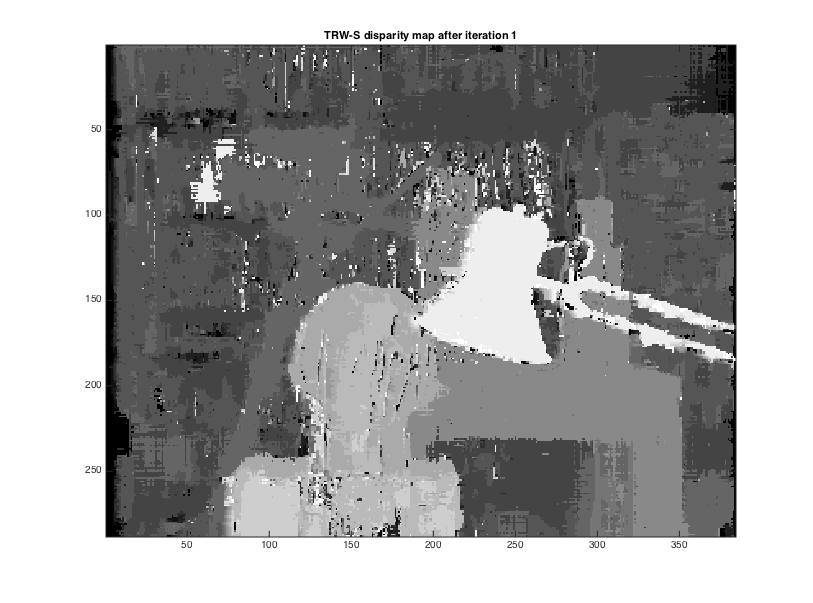
\includegraphics[scale=0.4]{dispmap.png}
		\caption{Obtained disparity map after 1 iteration}
	\end{figure}
Our algorithm took too much time to converge in Matlab, so we onyl present the result after 1 iteration (all pixels have been reparametrized).
The result is good, but we still see horizontal and vertical stripe, due to the trees we chose.
	\begin{figure}[H]
		\centering
		%\noindent\includegraphics[scale=2]{images/hypnoogle.png}
		\caption{Dual energy as a function of iterations}
	\end{figure}
	
		\begin{figure}[H]
		\centering
		%\noindent\includegraphics[scale=2]{images/hypnoogle.png}
		\caption{Energy as a function of iterations}
	\end{figure}

\end{document}